\section{Path}

The class Path represents the road that the mobs walk along. Each track has a unique path. Path contains a list of coordinates for all checkpoints of the road. A checkpoint is a point where the direction of the path changes. 

The Path in itself is not visible to the user, but the background image of the track contains a visual representation of it. The path is used by the two classes Mob and GameView. Mobs use it when they update their position on the game field. They use the coordinates to calculate in which direction they should move. GameView uses the path to calculate where the user can place towers, since the user is not allowed to place towers on the path.

The Path class is implemented as a singleton, so when the track is changed, the Path object is just reset and reused. The Path object is, just like the MobFactory object, first initialized when the player chooses a track from the progression map. The Path and MobFactory singletons are almost identical in their structure, but they handle different kinds of data.

When the path is initialized, information is read from an XML-file called initpaths. It is structured using one array for every track, where every item represents a checkpoint coordinate. Figure ~\ref{fig:codeExInitPathXML} shows the structure of initpath.

%-----
%- Code snippet initpath.xml
%-----
\begin{figure}[htb]

\begin{small}
\verbatiminput{code/initpathXML.java}
\end{small}

\caption{Caption}
\label{fig:codeExInitPathXML}

\end{figure}
%-----

The initiation contains two nested loops that iterate over every array tag and every item tag. The data is saved in an ArrayList, where every element is an ArrayList of coordinates (Figure  ~\ref{fig:dataStructurePath}).

%----
%- Image datastructure path
%----
\begin{figure}[here]

\begin{center}
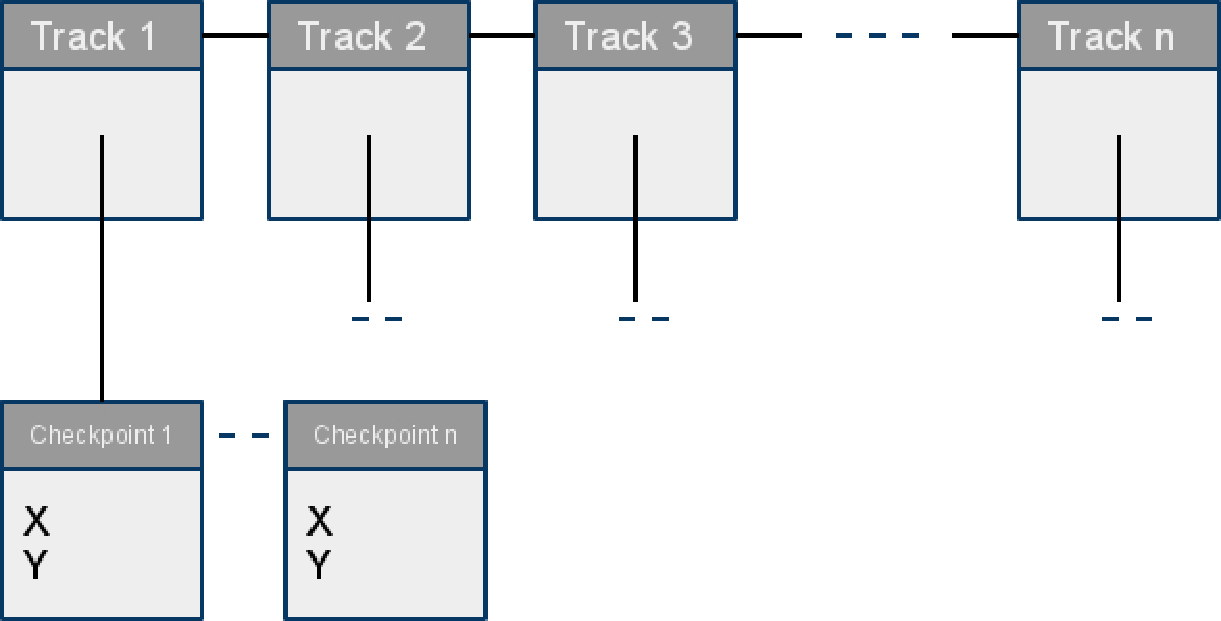
\includegraphics[scale=0.5]{pics/chapters/chapter4/pathlist2}
\end{center}

\caption{Caption}
\label{fig:dataStructurePath}
\end{figure}
%----
